\documentclass[landscape,a4paper]{article}
\usepackage[margin=1cm]{geometry}
\usepackage{tikz}
\pagestyle{empty}

\begin{document}
\centering
\newcommand{\steplength}{30}
\newcommand{\archlength}{1.6cm}
\newcommand{\drawarch}[1]{\draw[color=black,fill=black] (2*#1:\archlength) arc(2*#1:2*#1+\steplength:\archlength) 
	-- (0, 0) -- (2*#1:\archlength); }
%\newcommand{\drawdot}{\draw[fill=black] (0, 0) circle (0.75mm);}
\newcommand{\drawdot}{}
\newcommand{\draworder}[1]{\draw (0, -2.2) node {n = #1};}
\begin{tikzpicture}
\begin{scope}
\renewcommand{\steplength}{180}
\foreach \n in {0}{\drawarch{\n}}
\end{scope}
\begin{scope}[xshift=4cm]
\renewcommand{\steplength}{90}
\foreach \n in {0, \steplength, ..., 179}{\drawarch{\n}}
\end{scope}
\begin{scope}[xshift=8cm]
\renewcommand{\steplength}{60}
\foreach \n in {0, \steplength, ..., 179}{\drawarch{\n}}
\end{scope}
\begin{scope}[xshift=12cm]
\renewcommand{\steplength}{45}
\foreach \n in {0, \steplength, ..., 179}{\drawarch{\n}}
\end{scope}
\begin{scope}[xshift=16cm]
\renewcommand{\steplength}{36}
\foreach \n in {0, \steplength, ..., 179}{\drawarch{\n}}
\end{scope}
\begin{scope}[yshift=-4cm]
\renewcommand{\steplength}{30} % 180 / 6
\foreach \n in {0, \steplength, ..., 179}{\drawarch{\n}}
\end{scope}
\begin{scope}[yshift=-4cm, xshift=4cm]
\renewcommand{\steplength}{25.714} % 180 / 7
\foreach \n in {0, \steplength, ..., 179}{\drawarch{\n}}
\end{scope}
\begin{scope}[yshift=-4cm, xshift=8cm]
\renewcommand{\steplength}{22.5} % 180 / 8
\foreach \n in {0, \steplength, ..., 179}{\drawarch{\n}}
\end{scope}
\begin{scope}[yshift=-4cm, xshift=12cm]
\renewcommand{\steplength}{20} % 180 / 9
\foreach \n in {0, \steplength, ..., 179}{\drawarch{\n}}
\end{scope}
\begin{scope}[yshift=-4cm, xshift=16cm]
\renewcommand{\steplength}{18} % 180 / 10
\foreach \n in {0, \steplength, ..., 179}{\drawarch{\n}}
\end{scope}
\end{tikzpicture}

\newpage
\begin{tikzpicture}[scale=0.8]
\foreach \orderOfFive in {0, ..., 3}
{
	\foreach \order in {1, ..., 5}
	{
		\begin{scope}[xshift=-4cm + \order*4cm, yshift=- \orderOfFive * 4cm]
			% Do calculation
			\pgfmathsetmacro{\steplength}{180 / (\order + 5*\orderOfFive)}%
			\foreach \n in {0, \steplength, ..., 179}{\drawarch{\n}}
		\end{scope}
	}
}
\end{tikzpicture}


\newpage
\renewcommand{\archlength}{5cm}
\begin{tikzpicture}
\newcommand\order{2}
		\begin{scope}
			% Do calculation
			\pgfmathsetmacro{\steplength}{180 / \order}%
			\foreach \n in {0, \steplength, ..., 179}{\drawarch{\n}}
		\end{scope}
\renewcommand\order{3}
		\begin{scope}[xshift=13cm]
			% Do calculation
			\pgfmathsetmacro{\steplength}{180 / \order}%
			\foreach \n in {0, \steplength, ..., 179}{\drawarch{\n}}
		\end{scope}
\end{tikzpicture}

\newpage
\begin{tikzpicture}
\newcommand\order{4}
		\begin{scope}
			% Do calculation
			\pgfmathsetmacro{\steplength}{180 / \order}%
			\foreach \n in {0, \steplength, ..., 179}{\drawarch{\n}}
		\end{scope}
\renewcommand\order{5}
		\begin{scope}[xshift=13cm]
			% Do calculation
			\pgfmathsetmacro{\steplength}{180 / \order}%
			\foreach \n in {0, \steplength, ..., 179}{\drawarch{\n}}
		\end{scope}
\end{tikzpicture}


\newpage
\begin{tikzpicture}
\newcommand\order{7}
		\begin{scope}
			% Do calculation
			\pgfmathsetmacro{\steplength}{180 / \order}%
			\foreach \n in {0, \steplength, ..., 179}{\drawarch{\n}}
		\end{scope}
\renewcommand\order{9}
		\begin{scope}[xshift=13cm]
			% Do calculation
			\pgfmathsetmacro{\steplength}{180 / \order}%
			\foreach \n in {0, \steplength, ..., 179}{\drawarch{\n}}
		\end{scope}
\end{tikzpicture}



\newpage
\renewcommand{\archlength}{5cm}
\begin{tikzpicture}
\newcommand\order{7}
		\begin{scope}
			% Do calculation
			\pgfmathsetmacro{\steplength}{180 / \order}%
			\foreach \n in {0, \steplength, ..., 149}{\drawarch{\n}}
		\end{scope}
\renewcommand\order{9}
		\begin{scope}[xshift=13cm]
			% Do calculation
			\pgfmathsetmacro{\steplength}{180 / \order}%
			\foreach \n in {0, \steplength, ..., 149}{\drawarch{\n}}
		\end{scope}
\end{tikzpicture}




\newpage
\renewcommand{\archlength}{4cm}
\begin{tikzpicture}
\newcommand\order{6}
		\begin{scope}
			% Do calculation
			\pgfmathsetmacro{\steplength}{180 / \order}%
			\foreach \n in {0, \steplength, ..., 149}{\drawarch{\n}}
		\end{scope}
\renewcommand\order{7}
		\begin{scope}[xshift=9cm]
			% Do calculation
			\pgfmathsetmacro{\steplength}{180 / \order}%
			\foreach \n in {0, \steplength, ..., 149}{\drawarch{\n}}
		\end{scope}
\renewcommand\order{8}
		\begin{scope}[yshift=9cm]
			% Do calculation
			\pgfmathsetmacro{\steplength}{180 / \order}%
			\foreach \n in {0, \steplength, ..., 149}{\drawarch{\n}}
		\end{scope}
\renewcommand\order{9}
		\begin{scope}[xshift=9cm, yshift=9cm]
			% Do calculation
			\pgfmathsetmacro{\steplength}{180 / \order}%
			\foreach \n in {0, \steplength, ..., 149}{\drawarch{\n}}
		\end{scope}
\end{tikzpicture}



\newpage
\renewcommand{\archlength}{4cm}
\begin{tikzpicture}
\newcommand\order{4}
		\begin{scope}
			% Do calculation
			\pgfmathsetmacro{\steplength}{180 / \order}%
			\foreach \n in {0, \steplength, ..., 119}{\drawarch{\n}}
		\end{scope}
\renewcommand\order{5}
		\begin{scope}[xshift=9cm]
			% Do calculation
			\pgfmathsetmacro{\steplength}{180 / \order}%
			\foreach \n in {0, \steplength, ..., 119}{\drawarch{\n}}
		\end{scope}
\renewcommand\order{6}
		\begin{scope}[yshift=9cm]
			% Do calculation
			\pgfmathsetmacro{\steplength}{180 / \order}%
			\foreach \n in {0, \steplength, ..., 129}{\drawarch{\n}}
		\end{scope}
\renewcommand\order{7}
		\begin{scope}[xshift=9cm, yshift=9cm]
			% Do calculation
			\pgfmathsetmacro{\steplength}{180 / \order}%
			\foreach \n in {0, \steplength, ..., 139}{\drawarch{\n}}
		\end{scope}
\end{tikzpicture}



\newpage
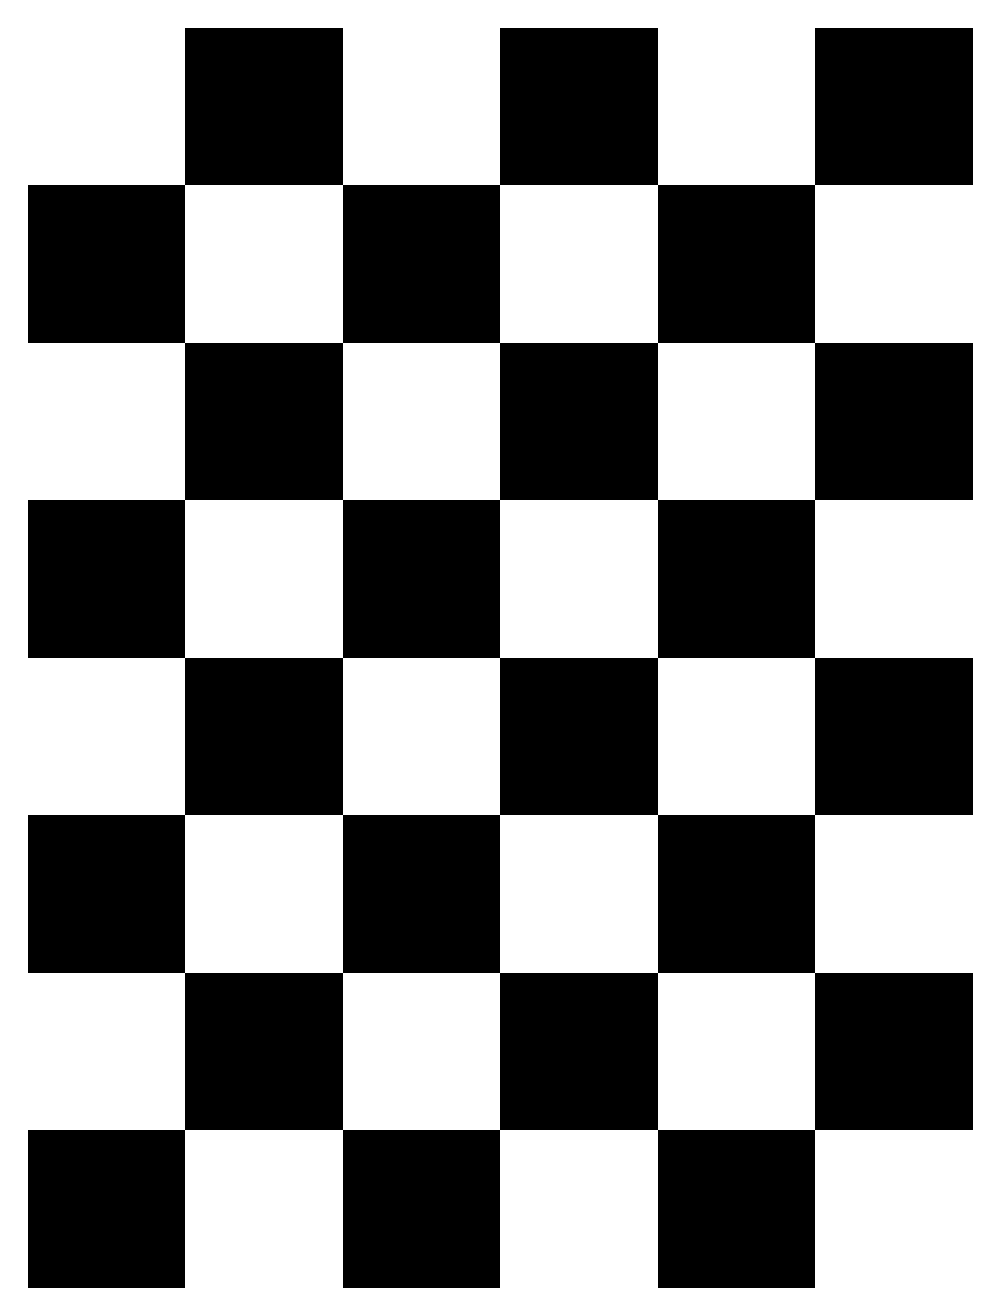
\begin{tikzpicture}[scale=2]
\fill (0, 0) rectangle ++(1, 1);
\fill (0, 2) rectangle ++(1, 1);
\fill (0, 4) rectangle ++(1, 1);
\fill (0, 6) rectangle ++(1, 1);
\fill (1, 1) rectangle ++(1, 1);
\fill (1, 3) rectangle ++(1, 1);
\fill (1, 5) rectangle ++(1, 1);
\fill (1, 7) rectangle ++(1, 1);
\fill (2, 0) rectangle ++(1, 1);
\fill (2, 2) rectangle ++(1, 1);
\fill (2, 4) rectangle ++(1, 1);
\fill (2, 6) rectangle ++(1, 1);
\fill (3, 1) rectangle ++(1, 1);
\fill (3, 3) rectangle ++(1, 1);
\fill (3, 5) rectangle ++(1, 1);
\fill (3, 7) rectangle ++(1, 1);
\fill (4, 0) rectangle ++(1, 1);
\fill (4, 2) rectangle ++(1, 1);
\fill (4, 4) rectangle ++(1, 1);
\fill (4, 6) rectangle ++(1, 1);
\fill (5, 1) rectangle ++(1, 1);
\fill (5, 3) rectangle ++(1, 1);
\fill (5, 5) rectangle ++(1, 1);
\fill (5, 7) rectangle ++(1, 1);
\end{tikzpicture}

\newpage
\renewcommand{\archlength}{10cm}
\begin{tikzpicture}
\newcommand\order{4}
		\begin{scope}
			% Do calculation
			\pgfmathsetmacro{\steplength}{180 / \order}%
			\foreach \n in {0, \steplength, ..., 179}{\drawarch{\n}}
		\end{scope}
		\draw[white, line width=1cm] (0, 0) circle (4cm);
\end{tikzpicture}

\newpage
\renewcommand{\archlength}{10cm}
\begin{tikzpicture}
\newcommand\order{6}
		\begin{scope}
			% Do calculation
			\pgfmathsetmacro{\steplength}{180 / \order}%
			\foreach \n in {0, \steplength, ..., 179}{\drawarch{\n}}
		\end{scope}
\end{tikzpicture}



\end{document}
